\documentclass{beamer}
\beamertemplatenavigationsymbolsempty
\usecolortheme{beaver}
\setbeamertemplate{blocks}[rounded=true, shadow=true]
\setbeamertemplate{footline}[page number]
%
\usepackage[utf8]{inputenc}
\usepackage[english,russian]{babel}
\usepackage{amssymb,amsfonts,amsmath,mathtext}
%\usepackage{subfig}
\usepackage[all]{xy} % xy package for diagrams
\usepackage{array}
\usepackage{multicol}% many columns in slide
\usepackage{hyperref}% urls
\usepackage{hhline}%tables
\usepackage{wrapfig}
% Your figures are here:
\graphicspath{ {fig/} {../fig/} }
\usepackage{subfigure}
\newtheorem{assumption}{Assumption}
\setbeamertemplate{theorems}[numbered]
%\setbeamertemplate{caption}[numbered]

%----------------------------------------------------------------------------------------------------------
\title[\hbox to 56mm{\href{https://arxiv.org/pdf/2002.03495}{A Diffusion Theory for Deep Learning Dynamics: Stochastic Gradient Descent Exponentially Favors Flat Minima}}]{\href{https://arxiv.org/pdf/2002.03495}{A Diffusion Theory for Deep Learning Dynamics: Stochastic Gradient Descent Exponentially Favors Flat Minima}}
\author[Veprikov Andrey]{Veprikov Andrey}
\institute{Bayesian multimodeling \\
Department of Intelligent Systems, MIPT}
\date{November 2024}

%----------------------------------------------------------------------------------------------------------
\begin{document}
%----------------------------------------------------------------------------------------------------------
\begin{frame}
\thispagestyle{empty}
\maketitle
\end{frame}
%-----------------------------------------------------------------------------------------------------
\begin{frame}{Stochastic Gradient Noise (SGN)}
    \begin{align}
    \label{eq:SGDD}
    \theta_{t+1}  = \theta_{t} -  \eta \frac{\partial \hat{L}(\theta_{t},x)}{\partial \theta_{t}} =  \theta_{t} -  \eta \frac{\partial L(\theta_{t})}{\partial \theta_{t}} + \eta C(\theta_{t})^{\frac{1}{2}} \zeta_{t}.
    \end{align}
    $\bullet$ $\hat{L}(\theta)$ is the loss of one minibatch
    
    $\bullet$ $\zeta_{t}$ is the noise variable
    
    $\bullet$ $C(\theta)$ represents the gradient noise covariance matrix

    \vspace{3mm}

    In the literature there are two main approaches of modeling SGN:

    $\bullet$ Gaussian noise, $\zeta_{t}  \sim  \mathcal{N}(0,\,I) $. 
    
    $\bullet$ L\'evy noise (stable variables)
\end{frame}

\begin{frame}{The Stochastic Gradient Noise Analysis}
\setcounter{subfigure}{0}
\vspace{-3mm}
\begin{figure}
\centering
\subfigure[\tiny{``SGN" across parameters}]{\includegraphics[width =0.40\columnwidth ]{Pictures/NoiseHist_B30_Dim.pdf}} 
\subfigure[\tiny{L\'evy noise}]{\includegraphics[width =0.40\columnwidth ]{Pictures/NoiseHist_B30_Levy.pdf}}  

\vspace{-1mm}
\subfigure[\tiny{SGN across minibatches}]{\includegraphics[width =0.40\columnwidth ]{Pictures/NoiseHist_B30_Batch.pdf}} 
\subfigure[\tiny{Gaussian noise}]{\includegraphics[width =0.40\columnwidth ]{Pictures/NoiseHist_B30_Gaussian.pdf}} 
\end{figure}
\end{frame}

\begin{frame}{SGD Dynamics}
    The continuous-time ($\eta \to dt$) dynamics of SGD \eqref{eq:SGDD} is written as
    \begin{align*}
    d \theta = -  \frac{\partial L(\theta)}{\partial \theta} dt +  [2D(\theta)]^{\frac{1}{2}}  dW_{t},
    \end{align*}
    where $d W_{t} \sim  \mathcal{N}(0,Idt)$ and $D(\theta) = \frac{\eta}{2} C(\theta)$. 

\vspace{3mm}

    The associated Fokker-Planck Equation is written as
\begin{align}
\label{eq:FP}
 \frac{\partial P(\theta, t)}{\partial t}  = &   \nabla \cdot [P(\theta, t) \nabla L(\theta) ]  + \nabla \cdot \nabla D(\theta)  P(\theta, t) .
\end{align}

\vspace{3mm}

In standard Stochastic Gradient Langevin Dynamics (SGLD), the injected gradient noise is fixed and isotropic Gaussian, $D = I$.
\end{frame}

\begin{frame}{Formulating the SGN Covariance Matrix $C(\theta)$}
    \begin{align*}
    C(\theta) 
    &= \frac{1}{B} \left[\frac{1}{m} \sum_{j=1}^{m}  \nabla L(\theta, x_{j})  \nabla L(\theta, x_{j})^{\top} -  \nabla L(\theta)  \nabla L(\theta)^{\top}\right] 
    \\&\approx \frac{1}{Bm} \sum_{j=1}^{m}  \nabla L(\theta, x_{j})  \nabla L(\theta, x_{j})^{\top}
    \\&=
    \frac{1}{B} \mathrm{FIM}(\theta) \approx  \frac{1}{B} H(\theta). 
    \end{align*}

    \vspace{3mm}

    This approximately gives
    \begin{align*}
    D(\theta)  = \frac{\eta}{2} C(\theta)  =  \frac{\eta }{2 B} H(\theta).
    \end{align*}
\end{frame}

\begin{frame}{Empirical verification of $C(\theta) = H(\theta) / B$}
\setcounter{subfigure}{0}
\vspace{-3mm}
    \begin{figure}
\center
\subfigure[\tiny{Pretrained Model}]{\includegraphics[width =0.40\linewidth ]{Pictures/HC_Corr_B0.pdf}} 
\subfigure[\tiny{Pretrained Model}]{\includegraphics[width =0.40\linewidth ]{Pictures/HC_Corr_B1.pdf}}   

\vspace{-1mm}
\subfigure[\tiny{Random Model}]{\includegraphics[width =0.40\linewidth ]{Pictures/HC_Corr_B0_random.pdf}} 
\subfigure[\tiny{Random Model}]{\includegraphics[width =0.40\linewidth ]{Pictures/HC_Corr_B1_random.pdf}}  
\end{figure}
\end{frame}

\begin{frame}{Kramers Escape Problem}     
     $\bullet$ Sharp Valley $a_{1}$ 
     
     $\bullet$ Flat Valley $a_{2}$ 
     
     $\bullet$ Col b is the boundary between two valleys

     $\bullet$ Col $c$ locates outside of Valley $a_{1}$
     
     %What is the mean escape time for a particle governed by Equation \ref{eq:GLD} to escape from Sharp Valley $a_{1}$ to Flat Valley $a_{2}$?
\setcounter{subfigure}{0}
     \begin{figure}
\center
\subfigure[\small{1-Dimensional Escape}]{\includegraphics[width =0.49\linewidth ]{Pictures/Kramers_Landscape.pdf}} %
\subfigure[\small{High-Dimensional Escape}]{\includegraphics[width =0.49\linewidth ]{Pictures/landscape_hd.pdf}}
\end{figure}
\end{frame}

\begin{frame}{Definition of the mean escape time $\tau$}
    We apply Gauss's Divergence Theorem to the Fokker-Planck Equation \eqref{eq:FP} resulting in
\begin{align*}
 \nabla \cdot [P(\theta, t) \nabla L(\theta) ]  + \nabla \cdot \nabla D(\theta)  P(\theta, t) = \frac{\partial P(\theta, t)}{\partial t} =  - \nabla \cdot J(\theta, t),
\end{align*}
where $J$ is the probability current. 

\vspace{3mm}

The mean escape time is expressed as
\begin{align*}
\tau = \frac{1}{\gamma} = \frac{P(\theta \in V_{a} ) }{\int_{S_{a}} J \cdot dS}.
\end{align*}

$\bullet$ $P(\theta \in V_{a} ) = \int_{V_{a}} P(\theta) dV$ is the current probability inside Valley a

$\bullet$ $J$ is the probability current produced by the probability source $P(\theta \in V_{a} )$
\end{frame}

\begin{frame}{Assumptions}
    \begin{assumption}[The Second Order Taylor Approximation]
 \label{as:1}
 The loss function around critical points $\theta^{\star}$ can be approximately written as 
 \[ L(\theta) = L(\theta^{\star}) + g(\theta^{\star})(\theta - \theta^{\star}) + \frac{1}{2}(\theta -\theta^{\star})^{\top} H(\theta^{\star}) (\theta -\theta^{\star}).\]
\end{assumption} 
 \begin{assumption}[Quasi-Equilibrium Approximation]
  \label{as:2}
The system is in quasi-equilibrium near minima.
 \end{assumption}
  \begin{assumption}[Low Temperature Approximation]
   \label{as:3}
The gradient noise is small (low temperature). 
 \end{assumption}
\end{frame}

\begin{frame}{Results for SGLD}
     \begin{theorem}[SGLD Escapes Minima]
 \label{pr:SGLD}
 The loss function $L(\theta)$ is of class $C^{2}$ and n-dimensional. Only one most possible path exists between Valley a and the outside of Valley a. If Assumption \ref{as:1}, \ref{as:2}, and \ref{as:3} hold, and the dynamics is governed by SGLD, then the mean escape time from Valley a to the outside of Valley a  is
 \[ \tau = \frac{1}{\gamma}=   2\pi  \sqrt{ \frac{-  \det (H_{b}) }{  \det (H_{a})} }  \frac{1}{|H_{be}|} \exp\left(\frac{\Delta L}{D}\right) . \]
 \end{theorem}
\vspace{-3mm}
$\bullet$ $H_{a}$ and $H_{b}$ are the Hessians of the loss function at the minimum $a$ and the saddle point $b$ 

$\bullet$ $\Delta L = L(b) - L(a)$ is the loss barrier height

$\bullet$ $e$ indicates the escape direction

$\bullet$ $H_{be}$ is the eigenvalue of the Hessian $H_{b}$ corresponding to the escape direction

$\bullet$ $D$ is the diffusion coefficient, usually set to $1$ in SGLD
\end{frame}

\begin{frame}{Results for SGD Diffusion}
    \begin{theorem}[SGD Escapes Minima]
 \label{pr:SGD}
 The loss function $L(\theta)$ is of class $C^{2}$ and n-dimensional.  Only one most possible path exists between Valley a and the outside of Valley a. If Assumption \ref{as:1}, \ref{as:2}, and \ref{as:3} hold, and the dynamics is governed by SGD, then the mean escape time from Valley a to the outside of Valley a is
 \[ \tau = 2\pi  \frac{1}{|H_{be}|} \exp\left[ \frac{2 B \Delta L}{\eta } \left(\frac{s }{H_{ae}} + \frac{(1-s)}{|H_{be}|}\right)\right]   . \]
 \end{theorem}

$\bullet$ $s \in (0,1)$ is a path-dependent parameter

$\bullet$ $H_{ae}$ and $H_{be}$ are, respectively, the eigenvalues of the Hessians at the minimum $a$ and the saddle point $b$ corresponding to the escape direction $e$
\end{frame}

\begin{frame}{Empirical Analysis}
\setcounter{subfigure}{0}
    \begin{figure}
\centering
\subfigure[$- \log(\gamma) = \mathcal{O}( \frac{1}{k}) $]{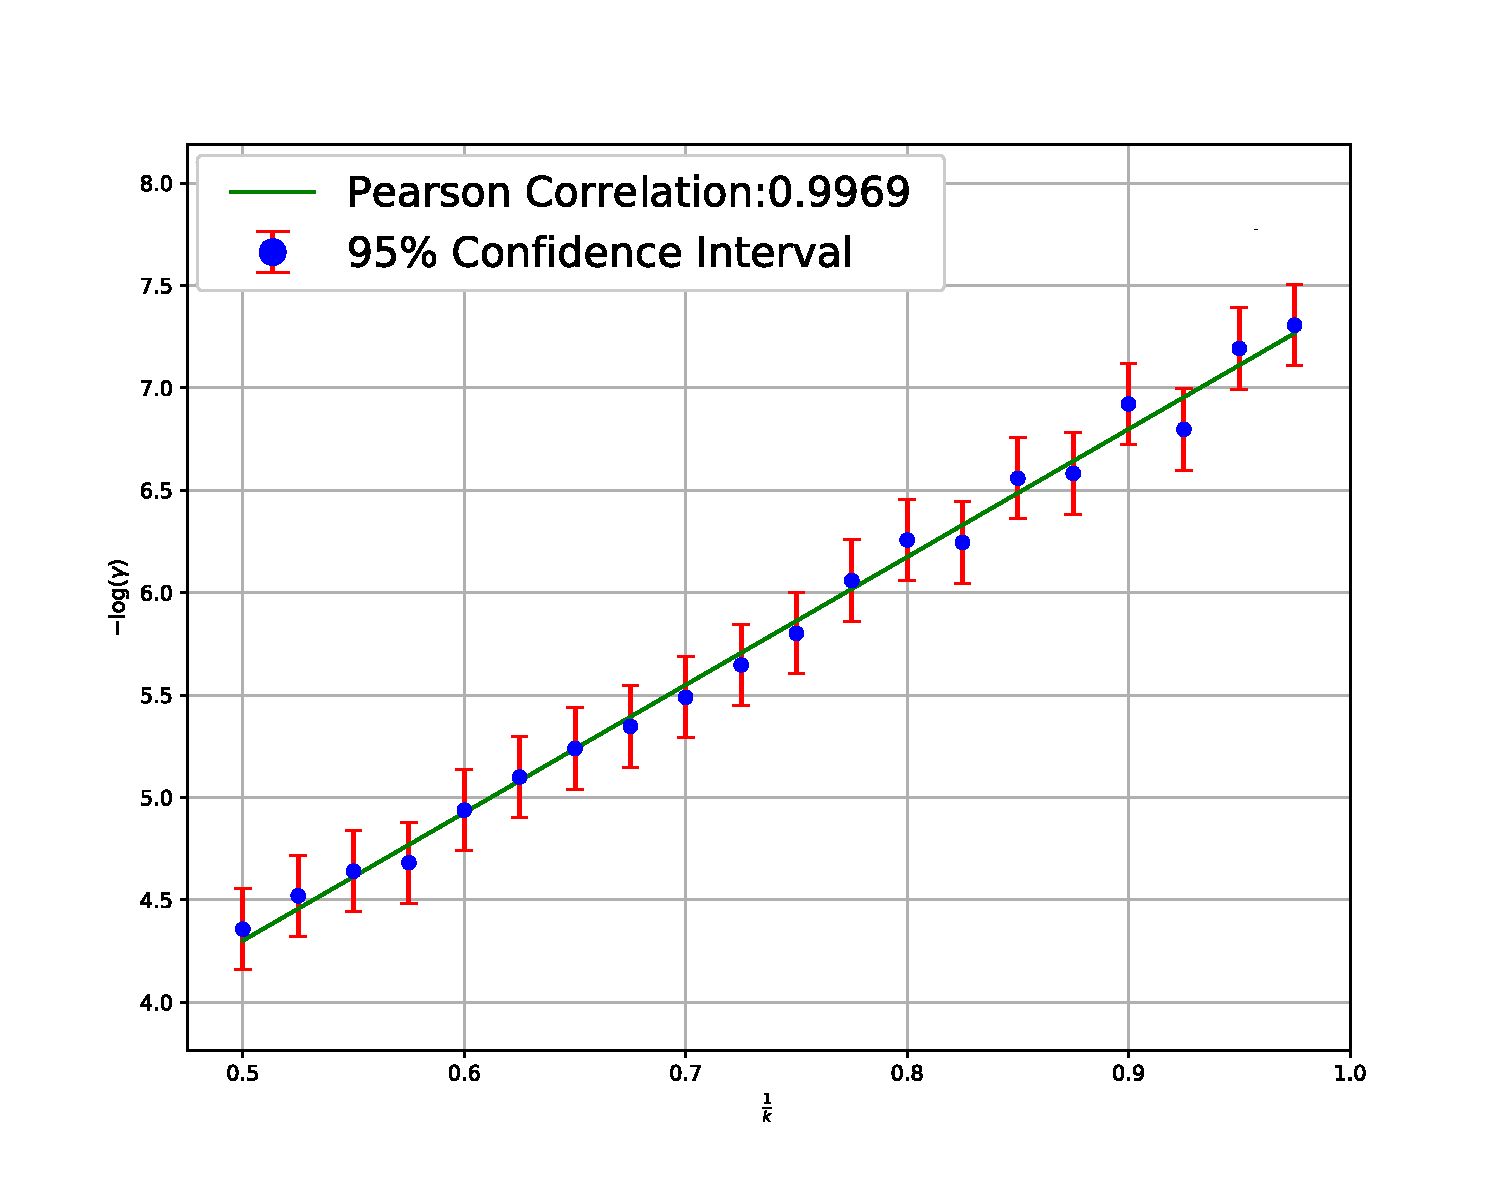
\includegraphics[width =0.32\linewidth ]{Pictures/escapingsgDST_ratio.pdf}} 
\subfigure[$- \log(\gamma) = \mathcal{O}( B ) $]{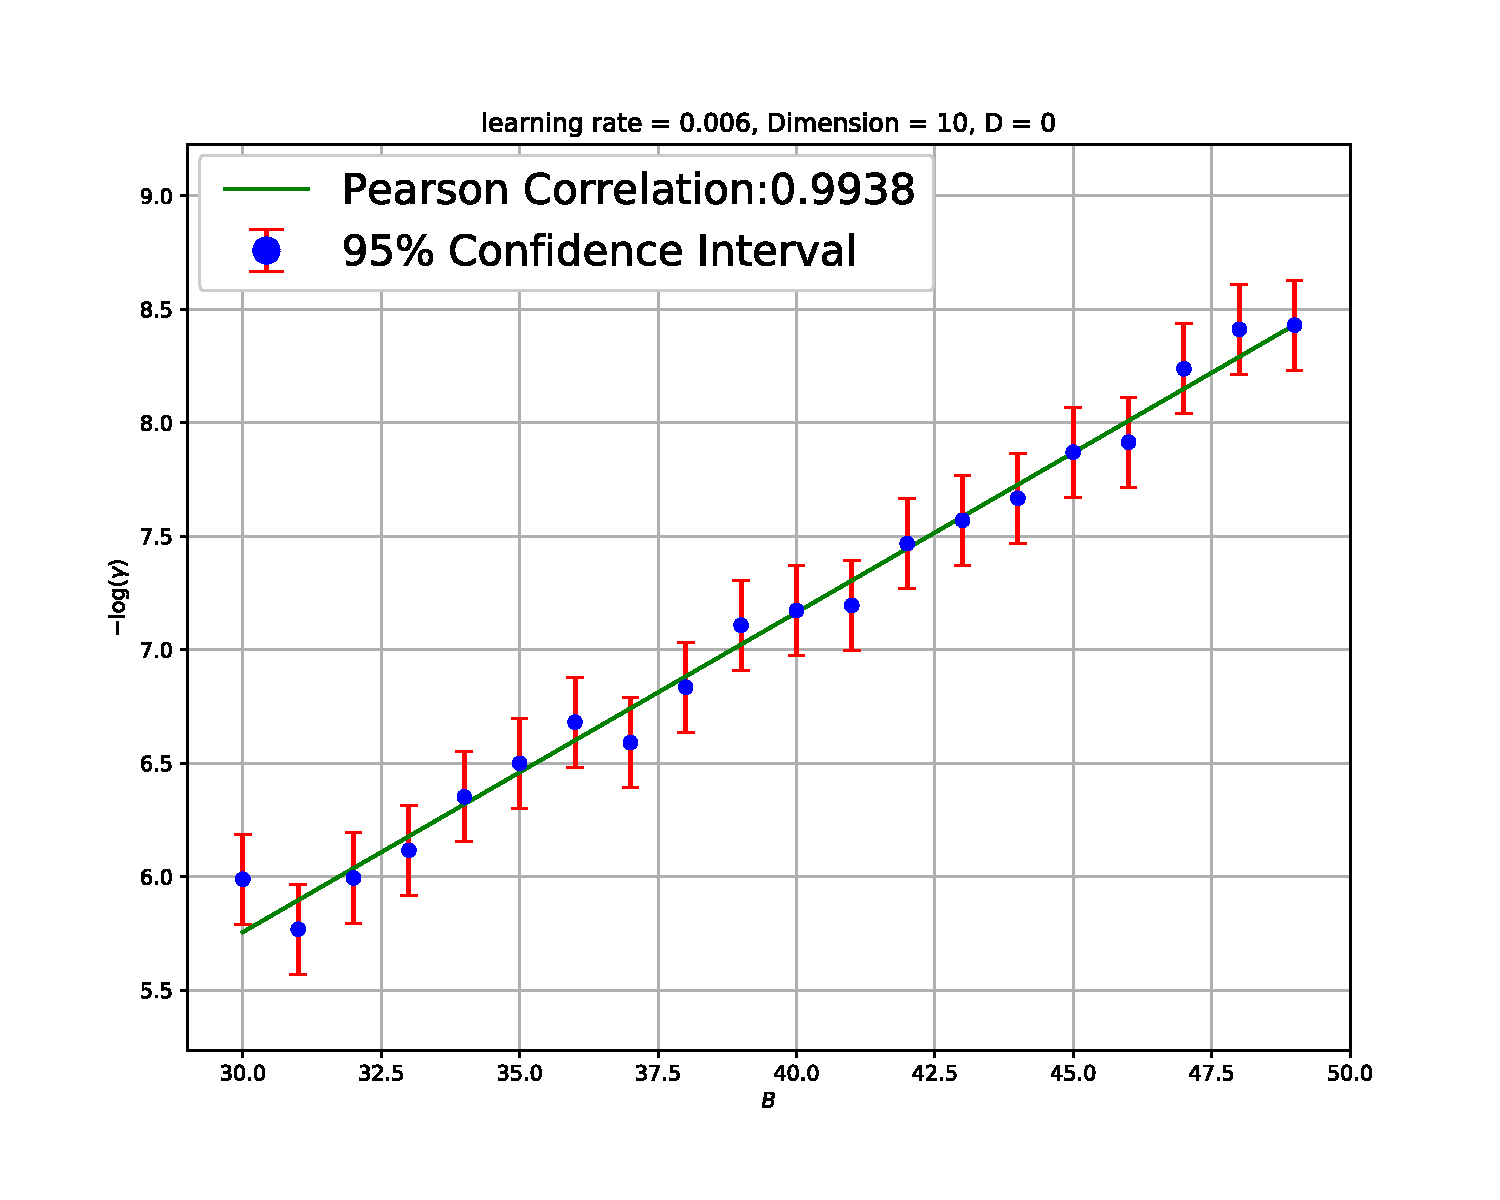
\includegraphics[width =0.32\linewidth ]{Pictures/escapingsgDST_B.pdf}}
\subfigure[$- \log(\gamma) = \mathcal{O}( \frac{1}{\eta} ) $]{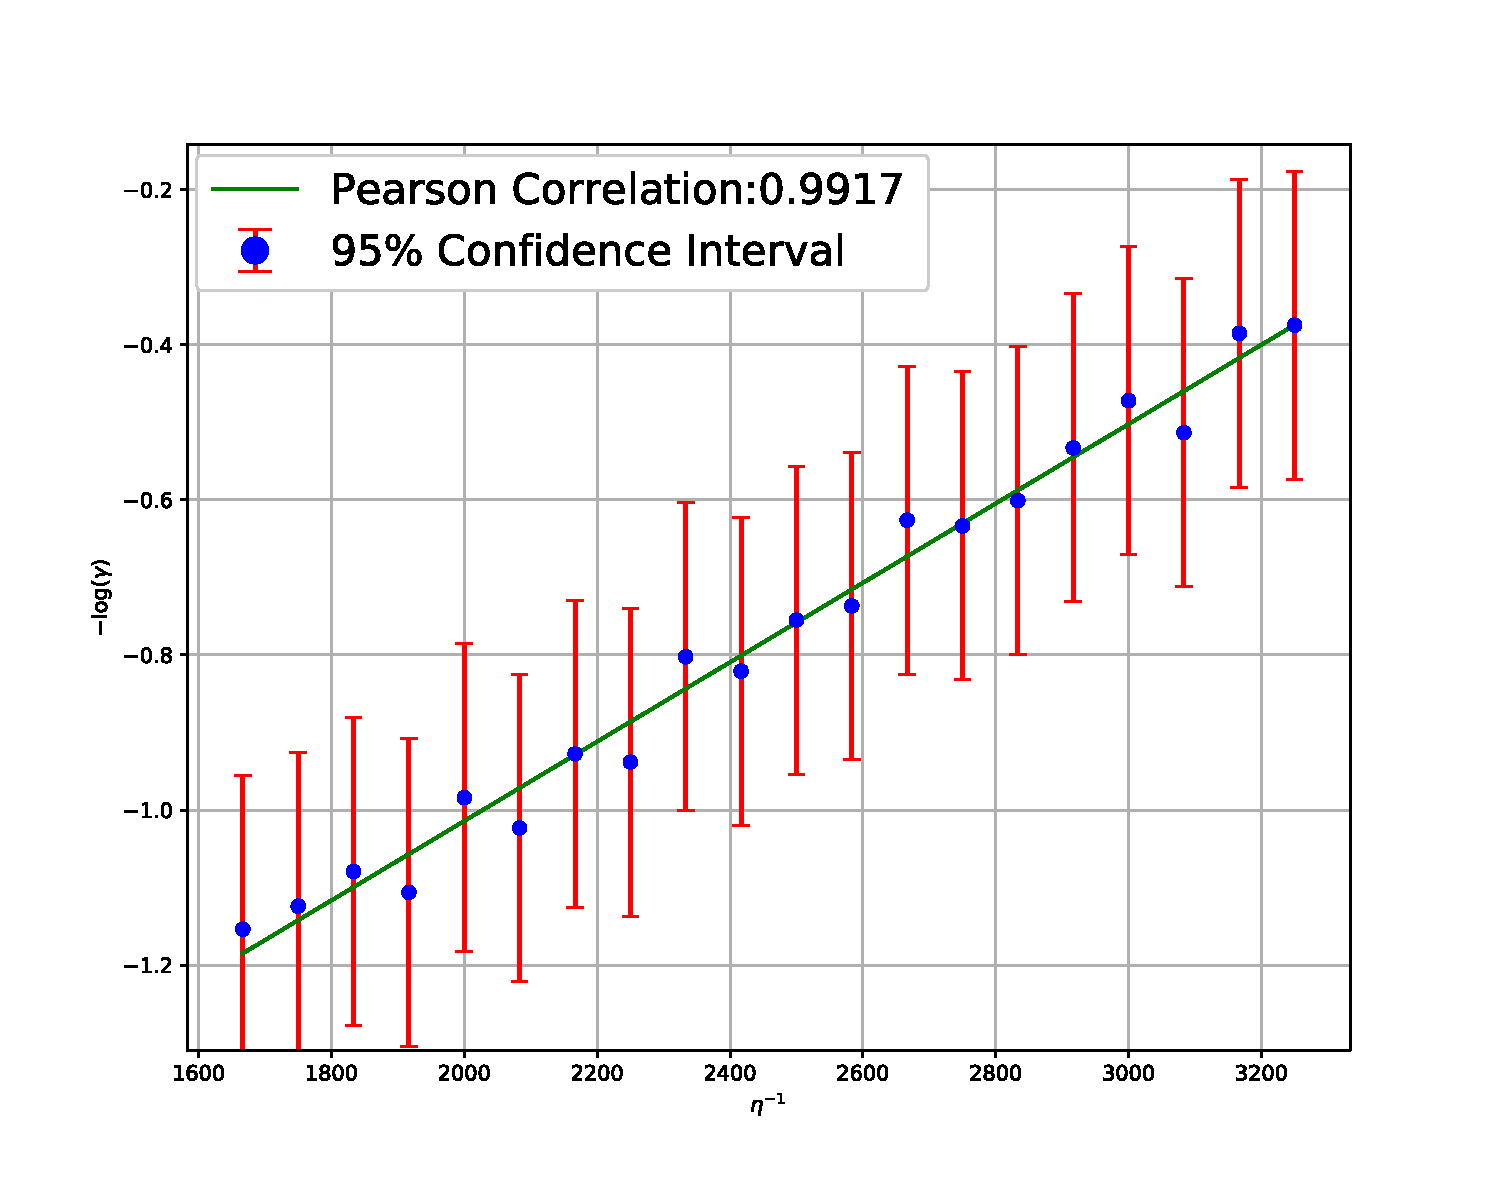
\includegraphics[width =0.32\linewidth ]{Pictures/escapingsgDST_LR.pdf}} 
\end{figure}

\begin{figure}
\centering
\subfigure[$- \log(\gamma) = \mathcal{O}( \frac{1}{k}) $]{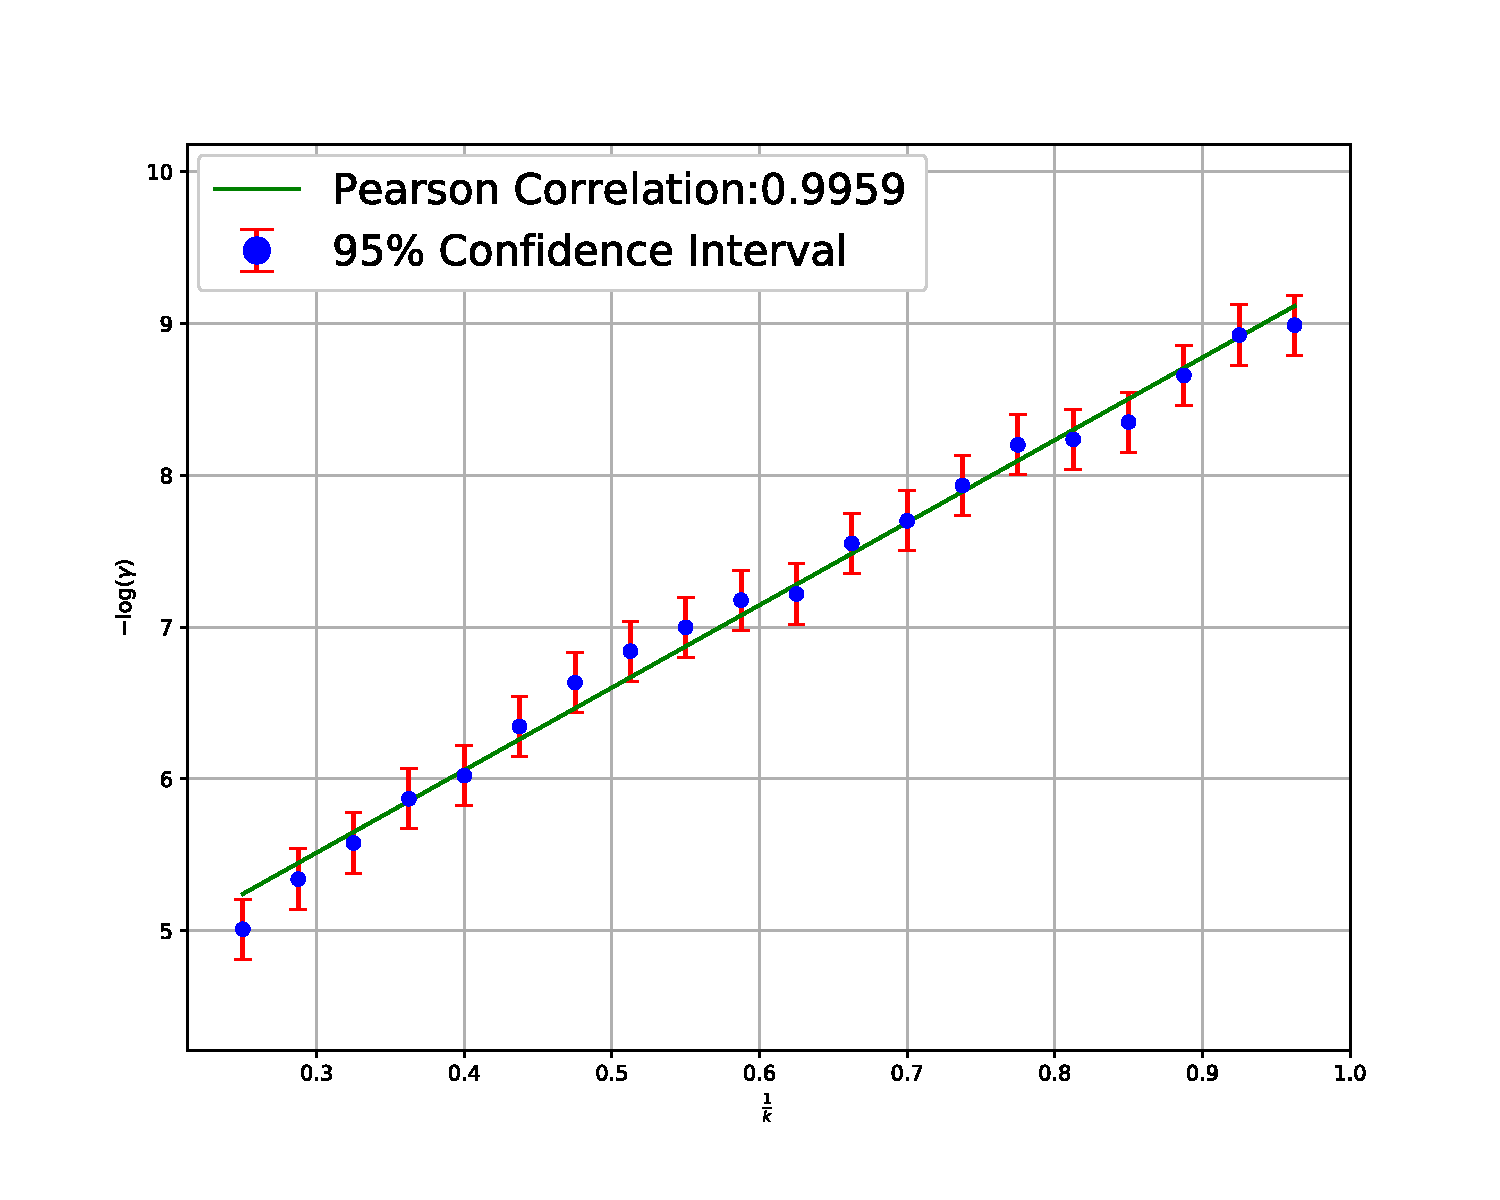
\includegraphics[width =0.32\columnwidth ]{Pictures/escapeD2Fcn_avila_ratio.pdf}} 
\subfigure[$- \log(\gamma) = \mathcal{O}( B ) $]{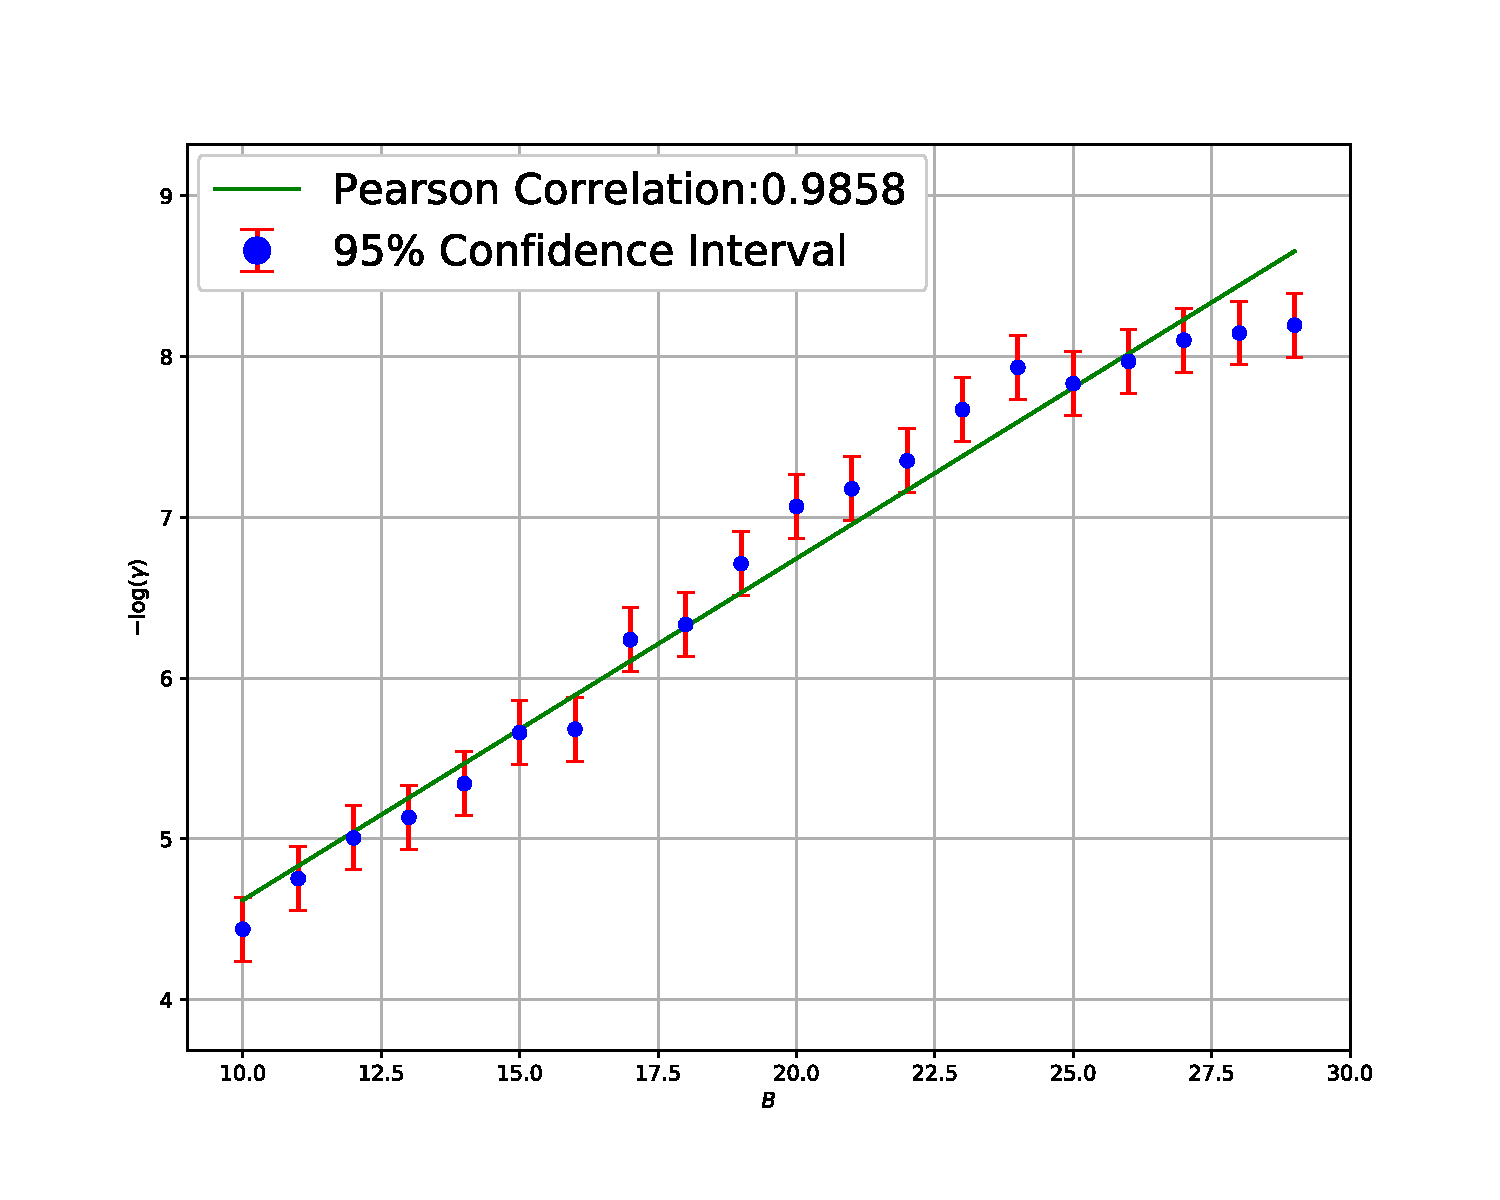
\includegraphics[width =0.32\columnwidth ]{Pictures/escapeD2Fcn_avila_B.pdf}}
\subfigure[$- \log(\gamma) = \mathcal{O}( \frac{1}{\eta} ) $]{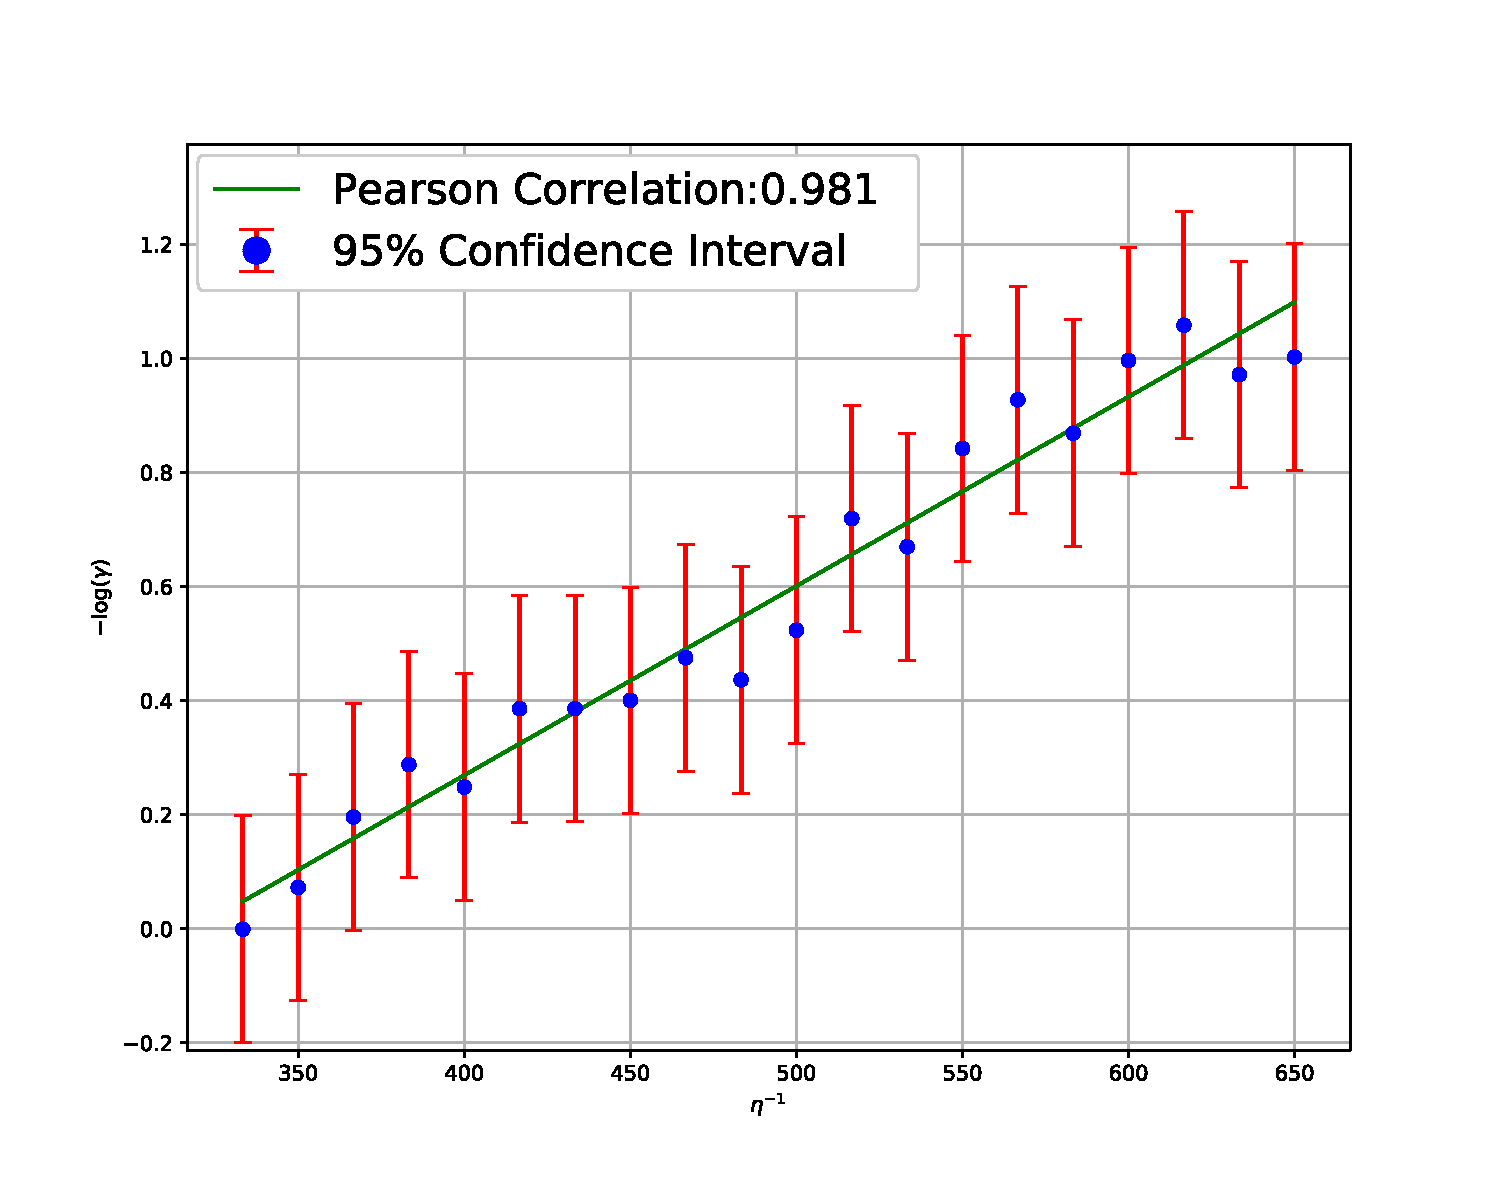
\includegraphics[width =0.32\columnwidth ]{Pictures/escapeD2Fcn_avila_LR.pdf}}
\end{figure}
\end{frame}

\begin{frame}{Conclusion}
    $\bullet$ SGD favors flat minima exponentially more than sharp minima 

    $\bullet$ The ratio of the batch size and the learning rate exponentially matters

    $\bullet$ Low dimensional diffusion

    $\bullet$ High-order effects
\end{frame}

% \begin{frame}{Список литературы}
%     \footnotesize
%     \bibliographystyle{apalike}
%     \bibliography{refs}
% \end{frame}
%----------------------------------------------------------------------------------------------------------
\end{document} 